% Author: Jiří Křištof <xkrist22@stud.fit.vutbr.cz>
% Author: Petr Češka <xceska05@stud.fit.vutbr.cz>


\documentclass[a4paper, 11pt]{article}


\usepackage[czech]{babel}
\usepackage[utf8]{inputenc}
\usepackage[left=2cm, top=3cm, text={17cm, 24cm}]{geometry}
\usepackage{times}
\usepackage{graphicx}
\usepackage[hyphens]{url}
\usepackage[unicode, colorlinks, hypertexnames=false, citecolor=red]{hyperref}

\begin{document}


	%%%%%%%%%%%%%%%%% Titulní stránka %%%%%%%%%%%%%%%%%
	\begin{titlepage}
		\begin{center}
			
\includegraphics[width=0.77\linewidth]{FIT_logo.pdf} \\

			\vspace{\stretch{0.382}}

			\Huge{Projektová dokumentace} \\
			\LARGE{\textbf{Modelování a simulace}} \\
			\Large{Téma 9 -- Diskrétní model z oblasti služeb a dopravy}
			\vspace{\stretch{0.618}}
		\end{center}

		\begin{minipage}{0.65 \textwidth}
			{\Large \today}
		\end{minipage}
		\hfill
		\begin{minipage}[r]{0.35 \textwidth}
			\Large
			\begin{tabular}{l l}
				\textbf{Jiří Křištof} & \textbf{(xkrist22)} \\
				Petr Češka & (xceska05) \\
			\end{tabular}
		\end{minipage}
	\end{titlepage}

	%%%%%%%%%%%%%%%%% Vlastní práce %%%%%%%%%%%%%%%%%

\section{Úvod}
V rámci projektu je řešen proces vyřizování objednávek jídel a jejich následná distribuce. Zejména z důvodu pandemie nemoci covid-19 se pro mnohá restaurační zařízení stal rozvoz jídla jedinou možností, jak jejich provoz nepřerušit. Smyslem projektu je zjistit, jaký způsob doručování jídel je pro restaurační provoz nejefektivnější a nejvýdělečnější. Díky zjištěným poznatkům je možné určit nejoptimálnější způsob doručování jídel pro restauraci.

\subsection{Autoři práce}
Na vypracování projektu se podíleli studenti FIT VUT v Brně Jiří Křištof (\texttt{xkrist22@stud.fit.vutbr.cz}) a Petr Češka (xceska05@stud.fit.vutbr.cz). 

\subsection{Zdroje}
Při řešení technické části projektu, jako sestavení modelu \cite[snímek 7]{IMS_course} a následná simulace \cite[snímek 8]{IMS_course}, byly využity zdroje z kurzu Modelování a simulace na FIT VUT. 

Fakta využívaná v rámci projektu byla získána pozorováním práce zaměstnanců provozovny rychlého občerstvení ROJ Kebab sídlící na adrese Skácelova 69, 612 00 Brno-Královo Pole.

V rámci projektu jsou dále využívána data o vozidlech obvykle realizující rozvozové služby \cite{car_peugeot, car_fiat}.

Pro zkoumání výdělečnosti doručování z hlediska restaurací využíváme výpočet ceny uváděný v prostředcích hromadného sdělování \cite{news}.

\subsection{Validita modelu}
Validita \cite[snímek 37]{IMS_course} byla ověřována při komunikaci se zaměstnanci výše zmíněné provozovny rychlého občerstvení. Validita byla dále ověřena pomocí srovnání experimentů \cite[snímek 9]{IMS_course} s realitou.

\section{Rozbor tématu, použité technologie}
Zákazníci si v průběhu dne telefonicky či online objednávají pokrmy připravované restaurací. Restaurace má určený počet kuchařů. Každý kuchař buď připravuje objednané jídlo, čeká na příjem objednávky, nebo si dopřává pauzu. Po připravení objednávky je jídlo buď doručeno kurýrem restaurace, nebo je po určitém čase předáno kurýrovi externí doručovací služby. Do nákladů restaurace jsou započítávány platy kuchařů a vlastních kurýrů, náklady na provoz vozidel a náklady spojené s externí doručovací službou.

Kurýr restauračního zařízení postupně rozváží zásilky. Při doručování jídla je možné využít dva různé typy vozidel. Prvním vozidlem je Peugeot Partner Combi; staitstiky o vozidle jsou uvedeny v tabulce \ref{tab:1}. Druhým testovaným vozidlem je Fiat Doblo; staitstiky o vozidle jsou uvedeny v tabulce \ref{tab:2}. Druh využívaného vozidla určuje náklady na vozidlo.

Vozidla při doručování spotřebovávají palivo z nádrže auta. Pokud je nádrž prázdná, řidič musí palivo znova natankovat. Tankování platí restaurační zařízení -- je započítáno do nákladů. Tankování dále způsobuje zpoždění kurýra restauračního zařízení. Dalším započítávaným nákladem restaurace jsou výdaje na provoz auta -- údržba apod. 

Při návratu kurýra do restaurace je čas návratu určen na základě pozorování jako 70 \% času cesty k zákazníkovi. 

Pokud je objednávka předána externí doručovací službě, pak si tato služba bere 30 \% z výdělku \cite{news} získaného danou objednávkou. 

\subsection{použité postupy}
Simulační model \cite[snímek 9]{IMS_course} je implementován programem v jazyce \texttt{C++} s využitím simulační knihovny \texttt{SIMLIB} \cite{SIMLIB}.
Knihovna \texttt{SIMLIB} je licencována pomocí \texttt{GNU LGPL} -- knihovnu je možné využít za předpokladu, že v této nebudou prováděny změny kódu.

Tato knihovna byla vybrána zejména díky možnosti jednoduché a přehledné implementace simulačního modelu. Knihovna je vhodná pro implementaci simulačních modelů systémů \cite[snímek 18]{IMS_course} s diskrétním chováním\cite[snímek 31]{IMS_course}, neboť poskytuje třídy a s nimi spojené metody pro realizaci využívaných konstruktů.

\subsection{Použité technologie}
V rámci projektu jsou využívány standardní knihovny jazyka \texttt{C++}. K překladu zdrojových souborů je využit nástroj \texttt{GNU Make}

Knihovna \texttt{SIMLIB} byla získána z oficiálních stránek \cite{SIMLIB}. V rámci projektu je využívána verze \texttt{3.07} vydaná dne 19, 10. 2018.

\section{Koncepce modelu}
Systém je modelován jako systém hromadné obsluhy \cite[snímek 136]{IMS_course}. Jako klíčové informace byly vybrány náklady a výdělky restauračního zařízení. 

\subsection{Popis konceptuálního modelu}
Konceptuální model \cite[snímek 41]{IMS_course} je vytvořen pomocí Petriho sítí \cite[snímek 123]{IMS_course}. Kuchaři jsou modelováni jako sklad \cite[snímek 146]{IMS_course} -- v systému může být více kuchařů, kteří mají jednu sdílenou frontu \cite[snímek 138]{IMS_course} objednávek. Do fronty objednávek může být vygenerován proces \cite[snímek 121]{IMS_course} s vyšší prioritou \cite[snímek 178]{IMS_course}, než standardní objednávky -- proces pauzy. Po vybrání procesu pauzy z fronty je simulována přestávka -- kuchař nevyřizuje žádnou objednávku. Pauza je generována po uplynutí určité doby, v Petriho síti je tato skutečnost modelována jako "počítadlo" -- při každé splněné objednávce je do místa \cite[snímek 123]{IMS_course} reprezentující čas vloženo určité množství procesů a po dovršení předem daného počtu procesů je provedena obsluha \cite[snímek 136]{IMS_course} pauzy.

Auta jsou modelována jako sklad -- v systému může být více aut, které mají sdílenou frontu objednávek. Do fronty může přijít prioritní proces představující nutnost natankovat palivo. Při obsluze procesu tankování není doručována žádná zásilka. V Petriho síti je toto modelováno jako "počítadlo" -- obdobně jako pro kuchaře jsou pro auta přidávány procesy do místa spotřebovaného paliva a ve chvíli, kdy je v tomto místu dostatek procesů, je proveden prioritní přechod \cite[snímek 128]{IMS_course} pro simulaci tankování paliva. 

Pokud procesy představující objednávky čekající ve frontě skladu kuchařů překročí určitou dobu čekání, pak tyto opouští systém. Pokud nebude objednávka vyřízena do předem určeného času, pak je tato zahozena. 

Proces objednávky obsloužený kuchařem následně vstupuje do místa, odkud může systém opustit časovaným přechodem \cite[snímek 132]{IMS_course}. Tento časovaný přechod představuje interval, po který objednávka čeká na kurýra restaurace. Opuštění systému tímto přechodem simuluje předání objednávky kurýrovi externí služby. Pakliže je ve skladu aut k dispozici auto, pak je zabrán 1 proces představující auto a je prováděna obsluha simulující přepravu objednávky. Po dokončení obsluhy opouští objednávka systém a auto se vrací do skladu aut, pokud není nutné provést tankování. 

\newpage

\subsection{Forma konceptuálního modelu}
Konceptuální model je reprezentován pomocí níže uvedené Petriho sítě.

\begin{figure}[h]
\centering
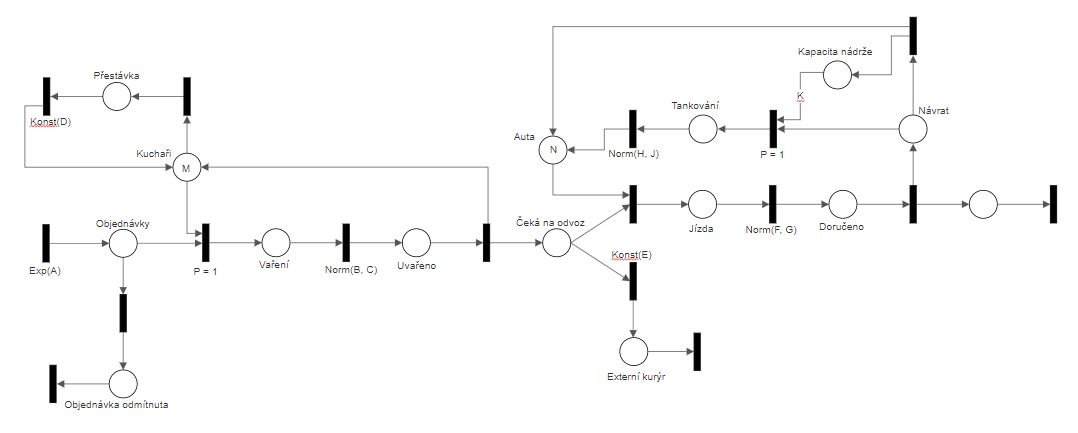
\includegraphics[width=16cm]{petriNet}
\caption{Konceptuální model ve formě Petriho sítě}
\label{fig:1}
\end{figure}

\section{Architektura simulačního modelu}
Simulační model je možné spouštět s parametry, které definují veškeré potřebné informace pro simulaci, jako čas simulace definovaný počtem dnů simulace a otevíracím a zavíracím časem restaurace nebo počty kuchařů a aut. Tato data se dále používají v modelu. Po provedení simulace jsou na standardní výstup vypsány statistiky o veškerých sledovaných vlastnostech modelu.

\subsection{Mapování konceptuálního modelu do simulačního modelu}
Jednotlivé prvky konceptuálního modelu jsou mapovány na model simulační.
 
 \subsubsection{Objednávky}
Procesy představující objednávky jsou implementovány třídou \texttt{Order}, která dědí ze třídy \texttt{Porcess} definované v knihovně \texttt{SIMLIB}. Metoda \texttt{Behavior} \cite[snímek 169]{IMS_course} pak definuje chování procesu. Časované přechody, které je možné přerušit příchodem procesu kuchaře do skladu kuchařů je modelována s pomocí cyklického vkládání události aktivace procesu \cite[snímek 169]{IMS_course} do kalendáře událostí \cite[snímek 173]{IMS_course} a následnou kontrolou počtu kuchařů či aut v daném skladu. 

Procesy objednávek jsou generovány pomocí metody implementované v rámci třídy \texttt{Shift}. Po vygenerování procesu je další proces vygenerován za čas daný exponenciálním rozložením \cite[snímek 91]{IMS_course}, které má střed definováno parametrem získaným při spuštění simulace. Před generováním objednávky je kontrolován aktuální čas systému. Pakliže je tento čas, který je mapován do intervalu 0 až 24 hodin, tedy do času v rámci jednoho dne, mimo otevírací dobu restaurace, pak je odloženo další generování na čas otevření restauračního zařízení. Touto skutečností je modelováno uzavření restaurace, např. přes noc. 

\subsubsection{Kuchaři}
Sklad kuchařů je implementován pomocí objektu třídy \texttt{Store} \cite[snímek 184]{IMS_course} definované v knihovně \texttt{SIMLIB}. Každá objednávka může zabrat právě jednoho kuchaře. Počet kuchařů ve skladu je dán k tomu určeným parametrem. Kuchař může být zabrán také prioritním procesem \texttt{Pause}. Celý sklad kuchařů je vytvořen po zpracování parametrů z příkazové řádky a stejně jako tyto parametry je sklad dostupný z objektu třídy \texttt{input\_data}.

Proces reprezentující pauzu kuchaře je implementován pomocí třídy \texttt{Pause}. Tento proces se díky nastavené prioritě umístí na začátek fronty skladu kuchařů. Při obsluze je simulována pauza kuchařů. Proces je generován v metodě \texttt{Behavior} objektů \texttt{Order}. Objednávky sdílí třídní proměnnou představující počítadlo času. Toto počítadlo je nastaveno na předem určenou hodnotu, od které se postupně odečítá čas zpracovávání objednávek kuchaři. Pokud hodnota tohoto počítadla klesne pod 0, pak je vygenerován proces \texttt{Pause} a hodnota počítadla obnovena.

\subsubsection{Kurýrní auta}
Objekt třídy \texttt{data\_input} dále udržuje sklad aut. Objednávky, které jsou obsloužené kuchařem, se tak řadí do fronty skladu aut, kde se pokoušejí zabrat právě jedno auto ze skladu aut. Sklad aut je reprezentován objektem třídy \texttt{Store}. Do fronty aut jsou dále vkládány prioritní procesy třídy \texttt{Refuel} dědící z třídy \texttt{Process}. Tento proces reprezentuje nutnost natankování paliva do auta. Obsluha tohoto procesu simuluje zpoždění způsobené tankováním.

Uvedený proces třídy \texttt{Refuel} je generován v metodě \texttt{Behavior} objektu \texttt{Order}. Jednotlivé objednávky sdílí počítadlo paliva, které je při spuštění simulace inicializováno na hodnotu reprezentující plnou nádrž. Tato hodnota je závislá na vybraném typu vozidla. Při každé jízdě kurýrního auta je vypočítána spotřeba z času potřebného na doručení. Pokud počítadlo paliva klesne pod 0, pak je vygenerován proces třídy \texttt{Refuel} reprezentující nutnost natankování a tento je vložen do fronty skladu aut. 

Jelikož není potřeba rozlišovat procesy aut či kuchařů, tak není nutné dále rozlišovat, který proces vybere z fronty pauzu či tankování -- tento proces způsobí zpoždění a započítá náklady restaurace, ať jej obslouží kterýkoliv proces. 

\subsection{Sbírané statistiky}
Při simulaci jsou sbírány tyto informace:
\begin{itemize}
\item Délka směny kuchařů
\item Celkový počet objednávek
\item Celkový počet odmítnutých objednávek, které nebyly obslouženy kuchařem ve stanoveném časovém intervalu
\item Počet objednávek doručených kurýry restauračního zařízení a k tomu vážící se data -- průměrný, maximální a minimální čas doručení
\item Počet objednávek doručených kurýry externí služby a k tomu vážící se data -- průměrný, maximální a minimální čas doručení
\item Celkový počet pauz kuchařů
\item Celkový počet tankování
\item Příjmy a výdaje restaurace -- celkový výdělek za prodané jídlo, náklady na externí doručovatele, náklady na palivo a údržbu vozů, náklady na platy kuchařů a vlastních kurýrů
\item Z výše uvedených příjmů a nákladů je vypočten čistý zisk restaurace
\end{itemize}
Tyto statistiky jsou vypsány na standardní výstup. Statistiky byly dále využity při shrnutí simulačních experimentů \cite[snímek 165]{IMS_course} a ověřování validity porovnáním s realitou.

\section{Podstata simulačních experimentů a jejich průběh}
%TODO
\subsection{Postup experimentování}
%TODO
\subsection{Dokumentace experimentů}
%TODO

\section{Shrnutí simulačních experimentů a závěr}
%TODO

%%%%%%%%%%%%%%%%% Přílohy %%%%%%%%%%%%%%%%%

\section*{Přílohy}
\begin{table}[h]
\centering
\begin{tabular}{cc}
\textbf{Parametr} & \textbf{Hodnota}                                                                                   \\ \hline
spotřeba & 6,7l/100km \\ \hline
nádrž  & 60l \\ \hline                      
dojezd &  896km \\ \hline
palivo & diesel
\end{tabular}
\caption{Využívané parametry vozu Peugeot Partner Combi}
\label{tab:1}
\end{table}

\begin{table}[h]
\centering
\begin{tabular}{cc}
\textbf{Parametr} & \textbf{Hodnota}                                                                                   \\ \hline
spotřeba & 9,7l/100km \\ \hline
nádrž  & 22l \\ \hline
dojezd &  227km \\ \hline
palivo & CNG
\end{tabular}
\caption{Využívané parametry vozu Fiat Doblo}
\label{tab:2}
\end{table}

\begin{table}[h]
\centering
\begin{tabular}{lcc}
\textbf{PHM} & \textbf{Stanice} & \textbf{Cena}                                                                                   \\ \hline
Diesel & Globus, Brno & 25,80 Kč \\ \hline
CNG & DPMB, Brno & 27,50 Kč
\end{tabular}
\caption{Ceny pohonných hmot ke dni 3. 12. 2020}
\label{tab:3}
\end{table}


	%%%%%%%%%%%%%%%%% Citace %%%%%%%%%%%%%%%%%
\bibliography{doc} 
\bibliographystyle{czechiso}
\end{document}

